\documentclass[tikz]{standalone}

\usepackage{pgfplots}

\pgfplotsset{compat=1.17}

\begin{document}
	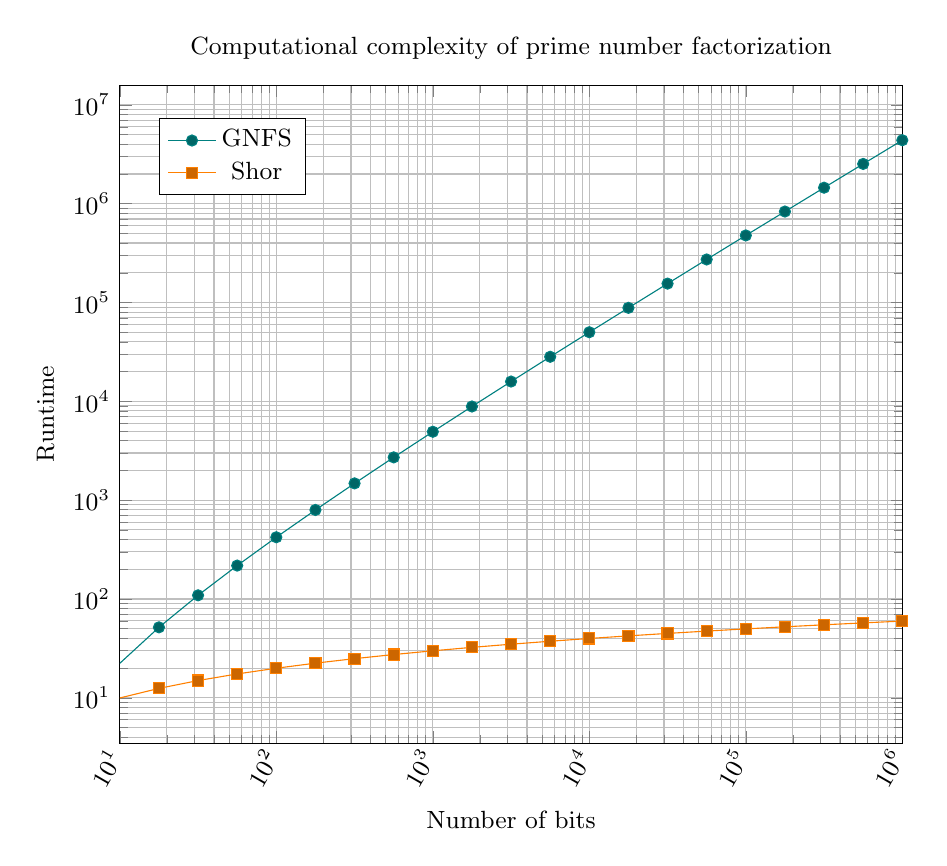
\begin{tikzpicture}[
		font=\small,
	]
		\begin{loglogaxis}[
			grid=both,
			width=0.95\linewidth,
			title={Computational complexity of prime number factorization},
			xmin=10,
			xmax=1e6,
			xticklabel style={/pgf/number format/1000 sep=, rotate=60, anchor=east},
			xlabel={Number of bits},
			ylabel={Runtime},
			log basis y=10,
			cycle list name=exotic,
			scaled x ticks=false,
			legend style={at={(0.05,0.95)}, anchor=north west,legend columns=1},
		]
			\addplot+[
				domain=1:1e6,
			] {exp(1.9*log2(x^(1/3)*log2(log2(x))^(2/3))};
			\addlegendentry{GNFS}
			\addplot+[
				domain=1:1e6,
			]
			{log2(x^3)};
			\addlegendentry{Shor}
		\end{loglogaxis}
	\end{tikzpicture}
\end{document}